\tikzset{every picture/.style={line width=0.75pt}} %set default line width to 0.75pt        

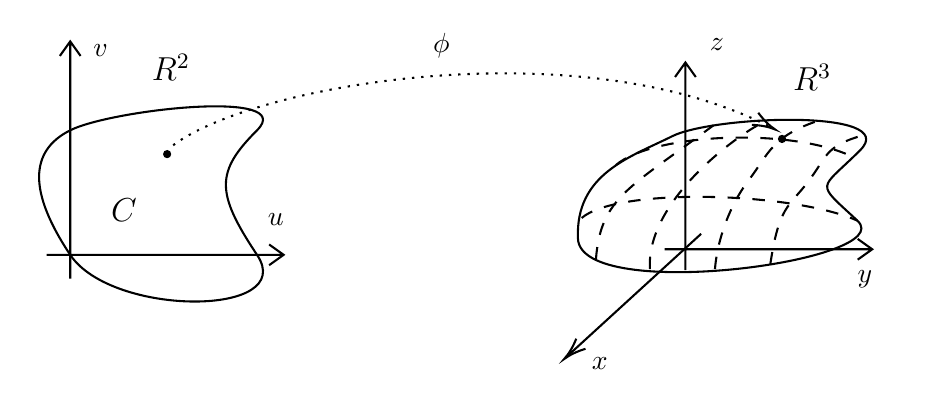
\begin{tikzpicture}[x=0.75pt,y=0.75pt,yscale=-1,xscale=1]
%uncomment if require: \path (0,310); %set diagram left start at 0, and has height of 310

%Shape: Polygon Curved [id:ds48992926630033473] 
\draw   (122,120) .. controls (142,110) and (232,100) .. (212,120) .. controls (192,140) and (192,150) .. (212,180) .. controls (232,210) and (142,210) .. (122,180) .. controls (102,150) and (102,130) .. (122,120) -- cycle ;
%Shape: Axis 2D [id:dp2965629103325713] 
\draw  (110.58,180) -- (224.82,180)(122,77.18) -- (122,191.42) (217.82,175) -- (224.82,180) -- (217.82,185) (117,84.18) -- (122,77.18) -- (127,84.18)  ;
%Shape: Axis 2D [id:dp5420346490627617] 
\draw  (408.4,177.33) -- (508.4,177.33)(418.4,87.33) -- (418.4,187.33) (501.4,172.33) -- (508.4,177.33) -- (501.4,182.33) (413.4,94.33) -- (418.4,87.33) -- (423.4,94.33)  ;
%Straight Lines [id:da7514964803526925] 
\draw    (425.96,169.89) -- (361.43,228.87) ;
\draw [shift={(359.96,230.22)}, rotate = 317.57] [color={rgb, 255:red, 0; green, 0; blue, 0 }  ][line width=0.75]    (10.93,-3.29) .. controls (6.95,-1.4) and (3.31,-0.3) .. (0,0) .. controls (3.31,0.3) and (6.95,1.4) .. (10.93,3.29)   ;
%Shape: Polygon Curved [id:ds6951808849645182] 
\draw   (411.96,122.89) .. controls (431.96,112.89) and (522.62,109.56) .. (502.62,129.56) .. controls (482.62,149.56) and (480.62,144.22) .. (501.29,163.56) .. controls (521.96,182.89) and (367.96,203.56) .. (366.62,172.22) .. controls (365.29,140.89) and (391.96,132.89) .. (411.96,122.89) -- cycle ;
%Curve Lines [id:da980778814237804] 
\draw  [dash pattern={on 4.5pt off 4.5pt}]  (375.29,182.22) .. controls (377.51,152.11) and (391.96,147.56) .. (431.96,117.56) ;
%Curve Lines [id:da5479602891033832] 
\draw  [dash pattern={on 4.5pt off 4.5pt}]  (401.29,186.89) .. controls (399.29,152.89) and (445.96,120.89) .. (454.62,116.89) ;
%Curve Lines [id:da6898603476087093] 
\draw  [dash pattern={on 4.5pt off 4.5pt}]  (432.62,186.89) .. controls (433.76,172.91) and (439.63,156.07) .. (449.07,143.78) .. controls (458.5,131.48) and (459.84,122.5) .. (483.96,114.89) ;
%Curve Lines [id:da9441978960398951] 
\draw  [dash pattern={on 4.5pt off 4.5pt}]  (459.29,184.56) .. controls (463.51,156.5) and (467.96,157.21) .. (477.4,144.92) .. controls (486.84,132.62) and (485.23,127.75) .. (503.9,122.42) ;
%Curve Lines [id:da5866336500737575] 
\draw  [dash pattern={on 4.5pt off 4.5pt}]  (368.4,162.25) .. controls (385.9,147.25) and (470.4,149.75) .. (501.29,163.56) ;
%Curve Lines [id:da6220068442378734] 
\draw  [dash pattern={on 4.5pt off 4.5pt}]  (384.9,136.75) .. controls (402.4,121.75) and (467.01,118.44) .. (497.9,132.25) ;
%Shape: Circle [id:dp15376632798085632] 
\draw  [fill={rgb, 255:red, 0; green, 0; blue, 0 }  ,fill opacity=1 ] (167.25,131.47) .. controls (167.25,130.68) and (167.9,130.03) .. (168.69,130.03) .. controls (169.49,130.03) and (170.13,130.68) .. (170.13,131.47) .. controls (170.13,132.27) and (169.49,132.92) .. (168.69,132.92) .. controls (167.9,132.92) and (167.25,132.27) .. (167.25,131.47) -- cycle ;
%Shape: Circle [id:dp39156470429151646] 
\draw  [fill={rgb, 255:red, 0; green, 0; blue, 0 }  ,fill opacity=1 ] (463.48,124.16) .. controls (463.48,123.36) and (464.13,122.71) .. (464.94,122.71) .. controls (465.74,122.71) and (466.39,123.36) .. (466.39,124.16) .. controls (466.39,124.97) and (465.74,125.62) .. (464.94,125.62) .. controls (464.13,125.62) and (463.48,124.97) .. (463.48,124.16) -- cycle ;
%Curve Lines [id:da06944123263869928] 
\draw  [dash pattern={on 0.84pt off 2.51pt}]  (171.6,127.2) .. controls (211.4,97.35) and (368.42,71.06) .. (460.22,118.87) ;
\draw [shift={(461.6,119.6)}, rotate = 208.05] [color={rgb, 255:red, 0; green, 0; blue, 0 }  ][line width=0.75]    (10.93,-3.29) .. controls (6.95,-1.4) and (3.31,-0.3) .. (0,0) .. controls (3.31,0.3) and (6.95,1.4) .. (10.93,3.29)   ;

% Text Node
\draw (215.67,158.4) node [anchor=north west][inner sep=0.75pt]    {$u$};
% Text Node
\draw (131.67,77.4) node [anchor=north west][inner sep=0.75pt]    {$v$};
% Text Node
\draw (499.87,186) node [anchor=north west][inner sep=0.75pt]    {$y$};
% Text Node
\draw (371.87,228) node [anchor=north west][inner sep=0.75pt]    {$x$};
% Text Node
\draw (428.67,74.4) node [anchor=north west][inner sep=0.75pt]    {$z$};
% Text Node
\draw (140.17,151.4) node [anchor=north west][inner sep=0.75pt]  [font=\large]  {$C$};
% Text Node
\draw (468.83,86.73) node [anchor=north west][inner sep=0.75pt]  [font=\large]  {$\mathbb{R}^{3}$};
% Text Node
\draw (159.83,81.9) node [anchor=north west][inner sep=0.75pt]  [font=\large]  {$\mathbb{R}^{2}$};
% Text Node
\draw (295.33,71.73) node [anchor=north west][inner sep=0.75pt]    {$\phi $};


\end{tikzpicture}
\caption{A map from $C$ to $\mathbb{R}^3$}